\def\fasterrcnn{
    Được lấy động lực từ những điểm yếu của mô hình Fast R-CNN \cite{girshick2015fast}, nhóm tác giả đã nghiên cứu và phát triển mô hình Faster R-CNN \cite{ren2015faster} với trung tâm là kiến trúc mô hình Region Proposal Network (gọi tắt là RPN).
    Mô hình RPN được kỳ vọng sẽ thay thế hoàn toàn các thuật toán như Selective Search \cite{uijlings2013selective} trong thành phần region proposals module \index{region proposals module} của các mô hình two-stage giải quyết bài toán object detection, hướng đến việc cải thiện không chỉ tốc độ của mô hình mà còn cải thiện về độ chính xác.

    \subsubsection{Kiến trúc mô hình RPN}
    Mô hình RPN nhận đầu vào là ảnh với kích thước bất kỳ và trả đầu ra là toạ độ của các khu vực và xác suất khu vực đó là đối tượng nào trong các lớp đối tượng \index{lớp đối tượng}.
    Nhằm tiết kiệm chi phí tính toán, mô hình RPN dùng chung phần feature extraction module \index{feature extraction module} với Fast R-CNN.

    \begin{figure}[H]
        \centering
        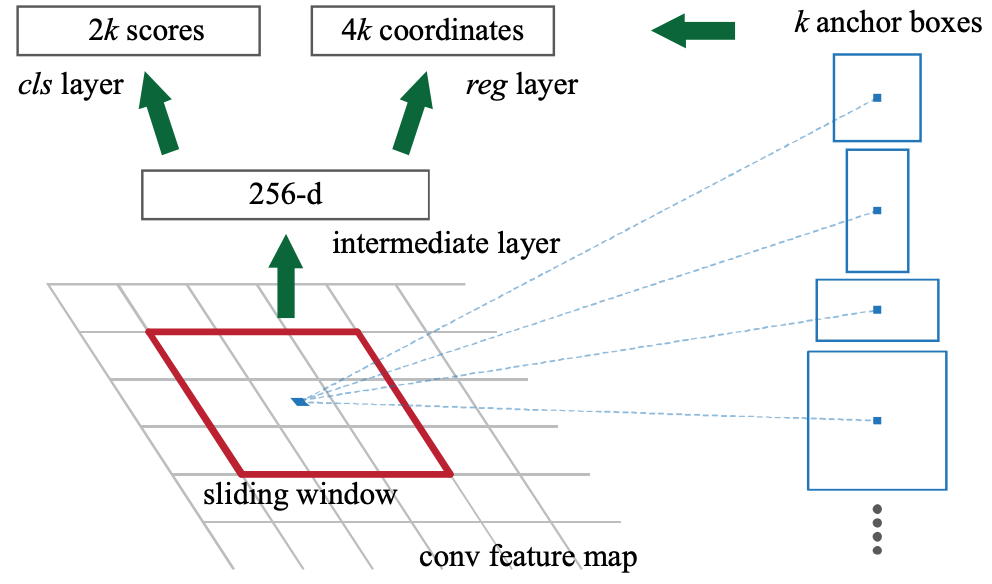
\includegraphics[width=9cm] {images/faster_rcnn_rpn}
        \caption{Kiến trúc mô hình RPN (Nguồn: \cite{ren2015faster})}
        \label{fig:faster_rcnn_rpn}
    \end{figure}
    
    \noindent
    Sau khi đưa ảnh qua feature extraction module \index{feature extraction module} và thu được một feature maps, mô hình RPN nhận đầu vào là feature maps \index{feature maps} này và trả đầu ra là các khu vực đề xuất gọi là các anchor \index{anchor}.
    Nhóm tác giả xây dựng phương pháp đề xuất các anchor \index{anchor} dựa trên kích thước và tỷ lệ giữa chiều dài và chiều rộng của anchor \index{anchor}.
    Cụ thể, mô hình RPN đưa feature maps \index{feature maps} qua một lớp Conv \index{lớp Conv} và thu được một feature maps \index{feature maps} mới có kích thước $W x H$.
    Từ đó, nhóm tác giả đề xuất ba kích thước của anchor \index{anchor} và ba tỷ lệ giữa chiều dài và chiều rộng của anchor \index{anchor} tạo ra chín anchor \index{anchor} với mỗi pixels \index{pixels} trên feature maps \index{feature maps} kích thước $W x H$.
    Tổng cộng trên toàn bộ feature maps \index{feature maps} kích thước $W x H$, ta thu được $W x H x 9$ anchor \index{anchor}.
    Các feature maps \index{feature maps} đại diện cho các anchor \index{anchor} này được tiếp tục đưa qua các lớp Conv \index{lớp Conv} để biến đổi về các feature maps \index{feature maps} mới có dạng $(W x H x 9) x 1$ đại diện cho xác suất anchor \index{anchor} đó là object và có dạng $(W x H x 9) x 4$ đại diện cho 4 toạ độ x của góc trái trên, y của góc trái trên, chiều dài và chiều rộng của bounding box \index{bounding box}.

    \noindent
    Một điểm mạnh của RPN so với các mô hình object detection thời bấy giờ đó chính là khả năng dự đoán được các object có kích thước khác nhau và tỷ lệ giữa chiều dài và chiều rộng khác nhau nhờ vào cách cấu hình của anchor \index{anchor}.

    \begin{figure}[H]
        \centering
        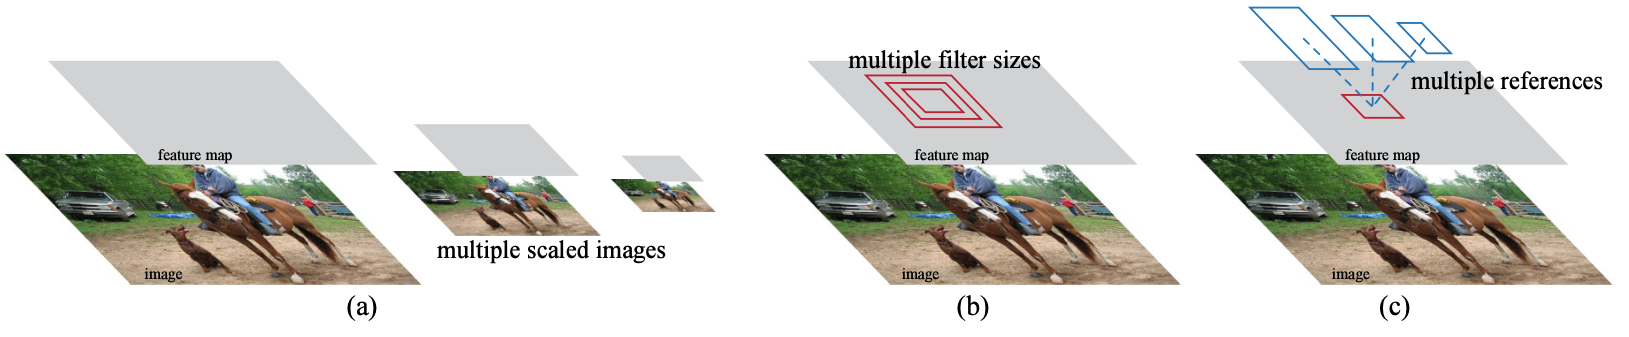
\includegraphics[width=15cm] {images/faster_rcnn_multi_scale_anchor}
        \caption{So sánh các kiến trúc xử lý vấn đề object có kích thước khác nhau và tỷ lệ giữa chiều dài và chiều rộng khác nhau (Nguồn: \cite{ren2015faster})}
        \label{fig:faster_rcnn_multi_scale_anchor}
    \end{figure}

    \noindent
    Một số kiến trúc đã được đề xuất ở thời điểm đó nhưng đều gặp phải rào cản về khối lượng tính toán lớn. \\
    - Kiến trúc đầu tiên là \textit{image/feature pyramids} sử dụng ảnh với nhiều kích thước khác nhau nhằm tạo ra feature maps \index{feature maps} có nhiều kích thước khác nhau.
    Kiến trúc này tốn rất nhiều chi phí tính toán do ta cần xử lý nhiều lần (thường là ba lần) với mỗi ảnh đầu vào khác nhau. \\
    - Kiến trúc thứ hai là \textit{pyramid of filters} đưa cùng một feature maps \index{feature maps} đầu vào qua nhiều khối Conv có kích thước của kernel khác nhau (thường là Conv với kernel 5x7 và Conv với kernel 7x5).
    Kiến trúc này tiết kiệm chi phí tính toán hơn một chút so với kiến trúc đầu tiên và thường được sử dụng kết hợp cùng với kiến trúc đầu tiên. \\
    - Kiến trúc cuối cùng là \textit{pyramid of anchors} được đề xuất trong RPN sử dụng nhiều anchor \index{anchor} với các kích thước khác nhau và tỷ lệ giữa chiều dài và chiều rộng khác nhau.
    Kiến trúc này chỉ tăng một lượng nhỏ chi phí tính toán nếu ta tăng số lượng anchor \index{anchor}, còn phần chi phí tính toán đối với feature maps \index{feature maps} vẫn được giữ nguyên. \\
    Phần cải tiến của RPN đối với object có kích thước khác nhau và tỷ lệ giữa chiều dài và chiều rộng khác nhau chỉ là những cải tiến tại thời điểm đó mà thôi.

    \subsubsection{Hàm loss và cách huấn luyện mô hình RPN}
    Để huấn luyện được mô hình RPN, nhóm tác giả gán cho mỗi anchor \index{anchor} một lớp groundtruth \index{groundtruth} và thiết lập hàm loss đối với từng anchor \index{anchor}.
    Nhóm tác giả gán lớp groundtruth \index{groundtruth} positive cho anchor \index{anchor} dựa theo hai cách sau: \\
    - Những anchor \index{anchor} có chỉ số IoU \index{IoU} lớn nhất đối với một groundtruth \index{groundtruth} bounding box \index{bounding box} được gán là anchor \index{anchor} positive. \\
    - Những anchor \index{anchor} có chỉ số IoU \index{IoU} lớn hơn 0.7 đối với một groundtruth \index{groundtruth} bounding box \index{bounding box} được gán là anchor \index{anchor} positive. \\
    Với hai cách như trên, một groundtruth \index{groundtruth} bounding box \index{bounding box} có thể gán được cho nhiều anchor \index{anchor} khác nhau.
    Ngoài ra, nhóm tác giả cũng gán lớp groundtruth \index{groundtruth} negative cho các anchor \index{anchor} không phải là positive và có chỉ số IoU \index{IoU} nhỏ hơn 0.3 đối với một groundtruth \index{groundtruth} bounding box \index{bounding box}. \\
    Từ đó, mô hình Faster R-CNN tối ưu hàm loss sau:

    \begin{equation}
        \label{eq:faster_rcnn_loss}
        L(\{p_i\}, \{t_i\}) = \frac{1}{N_{cls}}\sum_i L_{cls}(p_i, p^{*}_i) + \lambda\frac{1}{N_{reg}}\sum_i  p^{*}_i L_{reg}(t_i, t^{*}_i).
    \end{equation}

    \noindent
    trong đó: \\
    - \textit{i} là chỉ số của từng anchor \index{anchor}. \\
    - \textit{$p_i$} là xác suất mà anchor \index{anchor} chứa đối tượng. \\
    - \textit{$p^{*}_i$} là groundtruth \index{groundtruth} của anchor \index{anchor} (là 1 nếu anchor \index{anchor} đó được gán là chứa đối tượng, là 0 nếu anchor \index{anchor} đó được gán là không chứa đối tượng). \\
    - \textit{$t_i$} là vector gồm 4 giá trị đại diện cho toạ độ của khu vực mà mô hình RPN đề xuất. \\
    - \textit{$t^{*}_i$} là vector gồm 4 giá trị đại diện cho toạ độ của groundtruth \index{groundtruth} bounding box \index{bounding box} tương ứng với anchor \index{anchor} đó. \\
    Hàm loss trên gồm các thành phần: \\
    - \textit{$L_{cls}$}: là hàm loss phân lớp thông thường giúp xác định anchor \index{anchor} có chứa đối tượng hay không. \\
    - \textit{$L_{reg}$}: là hàm loss hồi quy đối với các anchor \index{anchor} positive, giúp tinh chỉnh toạ độ của khu vực mà mô hình đề xuất.
    Cụ thể, nhóm tác giả sử dụng $L_{reg}(t_i, t^{*}_i)=L_1(t_i - t^{*}_i)$ giống với hàm loss sử dụng trong mô hình Fast R-CNN \cite{girshick2015fast}.

    \noindent
    Mô hình RPN được thiết kế để có thể huấn luyện cùng với quá trình huấn luyện object detection từ đó giúp kết quả đề xuất khu vực trở nên chính xác hơn.
    Tuy nhiên, có một vấn đề nảy sinh khi sử dụng mô hình RPN cho việc đề xuất khu vực, đó là mô hình sẽ đề xuất ra nhiều các anchor \index{anchor} negative hơn rất nhiều so với số anchor \index{anchor} positive.
    Việc huấn luyện mô hình trên từng anchor \index{anchor} kết hợp với hiện tượng trên sẽ khiến cho tổng quan mô hình object detection bị mất cân bằng dữ liệu \index{mất cân bằng dữ liệu}.
    Ngoài ra, việc huấn luyện mô hình với toàn bộ số anchor \index{anchor} được đề xuất ra cũng sẽ khiến cho khối lượng tính toán lớn và thời gian kéo dài quá trình huấn luyện mô hình.
    Từ đó, nhóm tác giả đề xuất việc lựa chọn ngẫu nhiên 256 anchor \index{anchor} trên mỗi ảnh để thực hiện việc tính loss. Việc lựa chọn này giúp tỷ lệ anchor \index{anchor} positive và negative trở nên cân bằng hơn và giảm thiểu bởi những phần khối lượng tính toán dư thừa.

    \subsubsection{Sự kết hợp giữa mô hình RPN và Fast R-CNN}
    Nhóm tác giả cho rằng, việc huấn luyện mô hình RPN và Fast R-CNN cần phải diễn ra đồng thời, vì từ đó, việc chia sẻ chung thành phần backbone Conv mới trở nên hiệu quả.

    \begin{figure}[H]
        \centering
        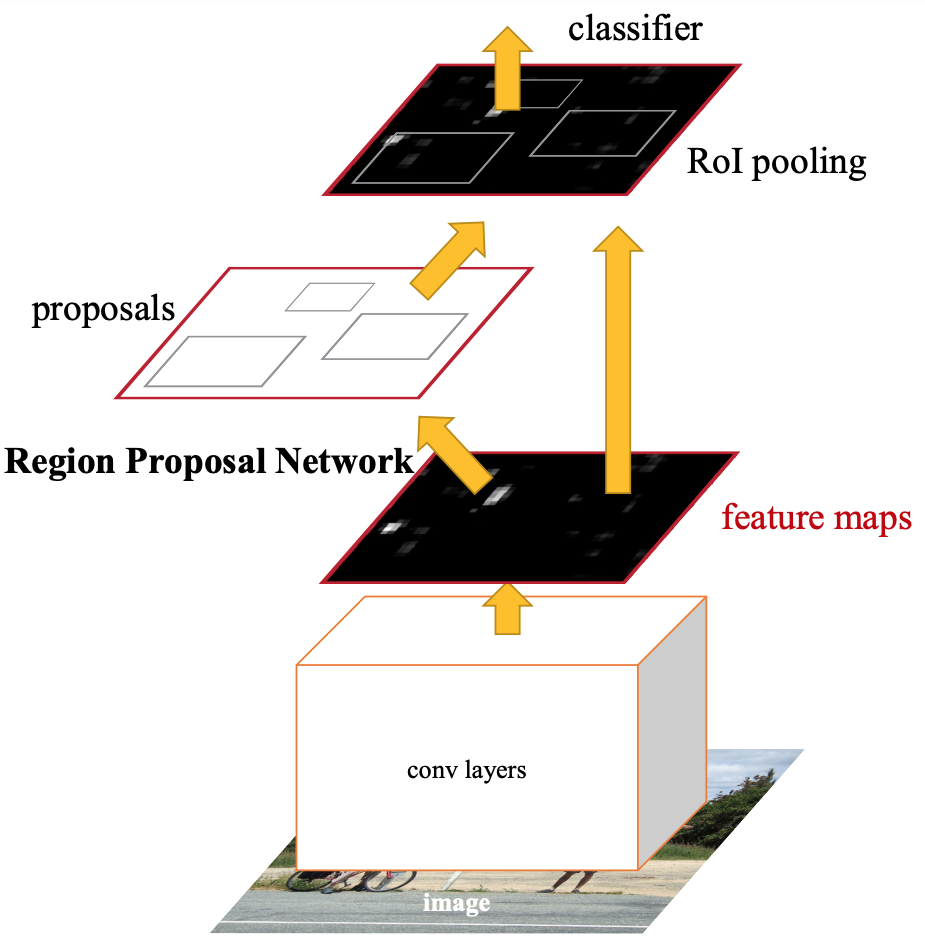
\includegraphics[width=10cm] {images/faster_rcnn_model}
        \caption{Toàn cảnh sự kết hợp của mô hình RPN và Fast R-CNN tạo ra mô hình Faster R-CNN (Nguồn: \cite{ren2015faster})}
        \label{fig:faster_model}
    \end{figure}

    \noindent
    Nhóm tác giả nêu ra ba phương án để huấn luyện mô hình RPN kết hợp với Fast R-CNN: \\
    - Cách 1: \textit{Alternating training}: Nhóm tác giả huấn luyện mô hình RPN trước sử dụng những hàm loss của RPN nói trên.
    Sau khi huấn luyện xong mô hình RPN, tác giả sử dụng những khu vực được đề xuất bởi RPN để huấn luyện mô hình Fast R-CNN.
    Mô hình backbone sau khi được huấn luyện bởi Fast R-CNN tiếp tục được sử dụng để huấn luyện mô hình RPN mới và vòng lặp này tiếp tục diễn ra cho đến khi kết quả của mô hình hội tụ. \\
    - Cách 2: \textit{Approximate joint training}: Phương pháp này kết hợp RPN và Fast R-CNN thành một mô hình duy nhất trong quá trình huấn luyện.
    Các khu vực được đề xuất bởi RPN được coi như là tất định đối với nhánh Fast R-CNN và khiến cho phương pháp huấn luyện này được gọi là \textit{approximate} bởi vì những thông tin từ nhánh Fast R-CNN sẽ không được cập nhật cho nhánh RPN.
    Quá trình backprop được thực hiện độc lập giữa RPN và Fast R-CNN, riêng phần backbone chung của RPN và Fast R-CNN được cập nhật theo giá trị hàm loss của cả RPN và Fast R-CNN.
    Phương pháp này đạt hiệu quả thấp hơn chút so với \textit{Alternating training} tuy nhiên thời gian huấn luyện được giảm 25 - 50\%. \\
    - Cách 3: \textit{Non-approximate joint training}: Phương pháp này cải thiện được vấn đề \textit{approximate} tồn đọng của \textit{Approximate joint training}.
    Tuy nhiên, để làm được điều này, nhóm tác giả cần tinh chỉnh lại lớp RoI pooling trong Fast R-CNN để có thể update cho cả các thành phần của mô hình Fast R-CNN và RPN.
    Điều này nằm ngoài nội dung của nghiên cứu này nên nhóm tác giả không đề cập kỹ hơn.

    \noindent
    Tóm lại, nhóm tác giả dựa vào phương pháp \textit{Alternating training} và thực hiện quá trình huấn luyện gồm 4 bước như sau: \\
    - Bước 1: Nhóm tác giả khởi tạo mô hình RPN với pretrained ImageNet và huấn luyện mô hình RPN. \\
    - Bước 2: Nhóm tác giả khởi tạo mô hình Fast R-CNN với pretrained ImageNet và huấn luyện mô hình Fast R-CNN với các khu vực được đề xuất bởi RPN. \\
    - Bước 3: Nhóm tác giả khởi tạo lại mô hình RPN nhưng sử dụng phần backbone đã được huấn luyện từ bước 2.
    Nhóm tác giả chỉ huấn luyện những lớp riêng của mô hình RPN và không cập nhật cho phần backbone. \\
    - Bước 4: Nhóm tác giả finetune lại những lớp riêng của mô hình Fast R-CNN với các khu vực được đề xuất bởi RPN và thu được mô hình Faster R-CNN cuối cùng. \\
    Nhóm tác giả cũng đã lặp lại 4 bước trên vài lần nhưng kết quả không thay đổi quá nhiều.

    % \subsubsection{Kết quả của mô hình Faster R-CNN}
    % Đầu tiên, trong hình \ref{fig:faster_rcnn_results_1}, kết quả của mô hình Fast R-CNN sử dụng RPN, backbone ZF-Net và dùng chung backbone giữa nhánh RPN và nhánh Fast R-CNN (\textbf{RPN+ZF, shared}) tốt hơn trên chỉ số mAP so sánh với việc sử dụng thuật toán Selective Search \textbf{SS} và EdgeBoxes \textbf{EB} trên bộ dữ liệu VOC 2007 test. Trong đó, số lượng khu vực được đề xuất trong quá trình huấn luyện được thống kê tại cột \textbf{\# boxes}, trong quá trình test được thống kê tại cột \textbf{\# proposals}.

    % \begin{figure}[H]
    %     \centering
    %     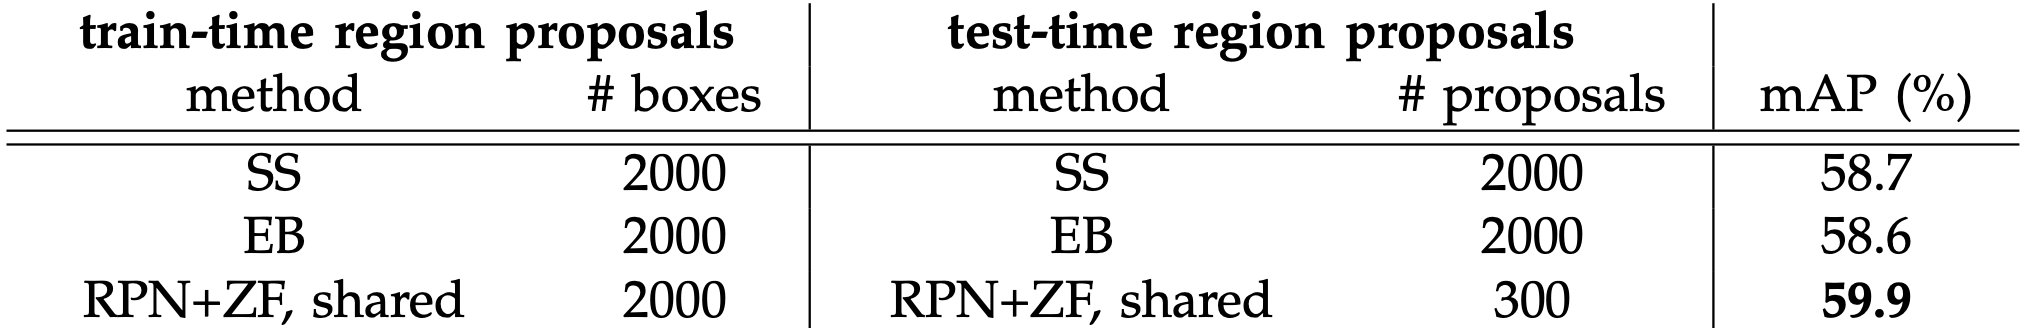
\includegraphics[width=10cm] {images/faster_rcnn_results_1}
    %     \caption{Kết quả của mô hình Fast R-CNN sử dụng RPN so sánh với việc sử dụng thuật toán Selective Search và EdgeBoxes trên bộ dữ liệu VOC 2007 test. (Nguồn: \cite{ren2015faster})}
    %     \label{fig:faster_rcnn_results_1}
    % \end{figure}

    % \noindent
    % Tiếp theo, trong hình \ref{fig:faster_rcnn_results_2}, nhóm tác giả so sánh kết quả của các mô hình Faster R-CNN (dùng backbone là VGG-16, ký hiệu là \textbf{RPN + VGG}) với mô hình Fast R-CNN sử dụng thuật toán Selective Search trên bộ dữ liệu VOC 2007 test nhưng với các bộ dữ liệu huấn luyện khác nhau. \\
    % - Cấu hình sử dụng riêng hai backbone khác nhau giữa nhánh RPN và nhánh Fast R-CNN: ký hiệu là \textbf{unshared} \\
    % - Cấu hình sử dụng chung backbone giữa nhánh RPN và nhánh Fast R-CNN: ký hiệu là \textbf{shared} \\
    % - Cấu hình sử dụng bộ dữ liệu huấn luyện là VOC07 trainval: ký hiệu là \textbf{07} \\
    % - Cấu hình sử dụng bộ dữ liệu huấn luyện là sự kết hợp giữa VOC07 trainval và VOC12 trainval: ký hiệu là \textbf{07+12} \\
    % - Cấu hình sử dụng bộ dữ liệu huấn luyện là sự kết hợp giữa VOC07 trainval, VOC12 trainval và bộ dữ liệu MS-COCO: ký hiệu là \textbf{COCO+07+12} \\
    % Trong đó, số lượng khu vực được đề xuất trong quá trình test được thống kê tại cột \textbf{\# proposals}. \\
    % Kết quả mô hình \textbf{RPN + VGG, unshared, 07} đạt chỉ số mAP là 68.5\%, tốt hơn so với 66.9\% của mô hình \textbf{SS, 07}.
    % Kết quả mô hình \textbf{RPN + VGG, shared, 07+12} đạt chỉ số mAP là 73.2\%, tốt hơn so với 70.0\% của mô hình \textbf{SS, 07+12}.
    % Và mô hình \textbf{RPN + VGG, shared, COCO+07+12} đạt chỉ số mAP cao nhất là 78.8\%, điều này khá dễ hiểu khi mô hình sử dụng nhiều dữ liệu huấn luyện hơn sẽ cho kết quả tốt hơn.

    % \begin{figure}[H]
    %     \centering
    %     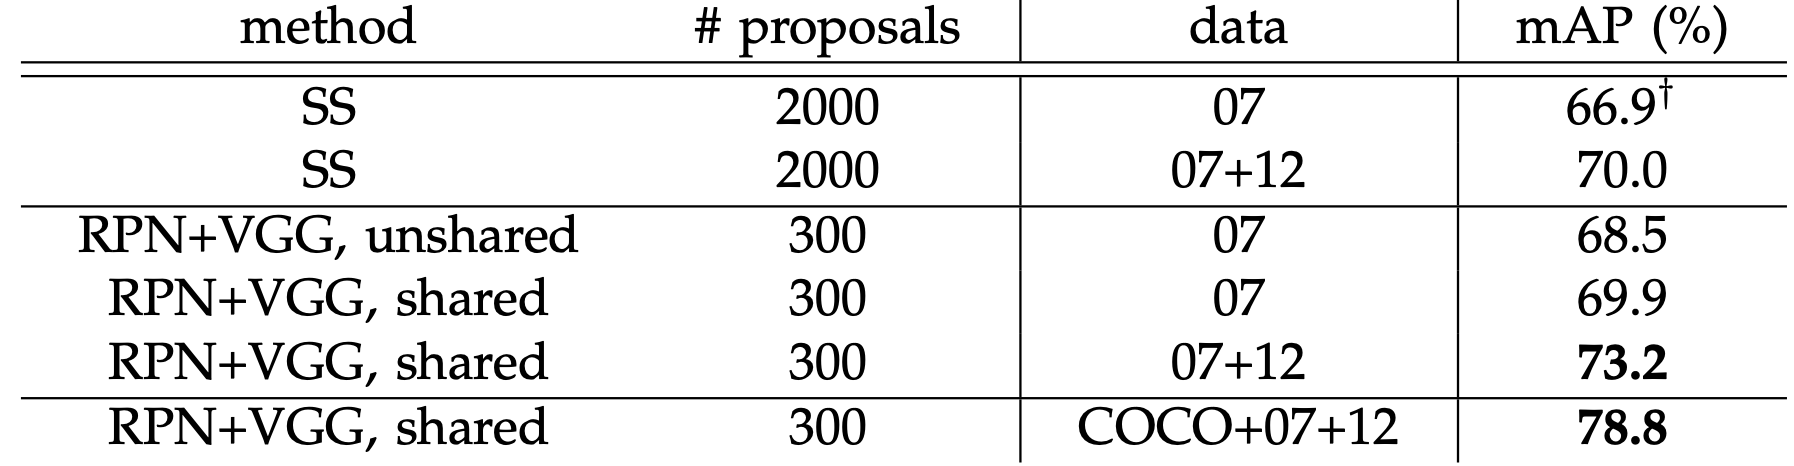
\includegraphics[width=10cm] {images/faster_rcnn_results_2}
    %     \caption{Kết quả của mô hình Fast R-CNN sử dụng RPN và backbone VGG-16 so sánh với mô hình Fast R-CNN sử dụng thuật toán Selective Search trên bộ dữ liệu VOC 2007 test với các bộ dữ liệu huấn luyện khác nhau. (Nguồn: \cite{ren2015faster})}
    %     \label{fig:faster_rcnn_results_2}
    % \end{figure}

    % \noindent
    % Tiếp theo, trong hình \ref{fig:faster_rcnn_results_3}, nhóm tác giả so sánh kết quả của các mô hình Faster R-CNN (dùng backbone là VGG-16, ký hiệu là \textbf{RPN + VGG}) với mô hình Fast R-CNN sử dụng thuật toán Selective Search trên bộ dữ liệu VOC 2012 test nhưng với các bộ dữ liệu huấn luyện khác nhau. \\
    % - Cấu hình sử dụng chung backbone giữa nhánh RPN và nhánh Fast R-CNN: ký hiệu là \textbf{shared} \\
    % - Cấu hình sử dụng bộ dữ liệu huấn luyện là VOC12 trainval: ký hiệu là \textbf{12} \\
    % - Cấu hình sử dụng bộ dữ liệu huấn luyện là sự kết hợp giữa VOC07 trainval+test và VOC12 trainval: ký hiệu là \textbf{07++12} \\
    % - Cấu hình sử dụng bộ dữ liệu huấn luyện là sự kết hợp giữa VOC07 trainval+test, VOC12 trainval và bộ dữ liệu MS-COCO: ký hiệu là \textbf{COCO+07+12} \\
    % Trong đó, số lượng khu vực được đề xuất trong quá trình test được thống kê tại cột \textbf{\# proposals}. \\
    % Kết quả mô hình \textbf{RPN + VGG, shared, 12} đạt chỉ số mAP là 67.0\%, tốt hơn so với 65.7\% của mô hình \textbf{SS, 12}.
    % Kết quả mô hình \textbf{RPN + VGG, shared, 07++12} đạt chỉ số mAP là 70.4\%, tốt hơn so với 68.4\% của mô hình \textbf{SS, 07++12}.
    % Và mô hình \textbf{RPN + VGG, shared, COCO+07++12} đạt chỉ số mAP cao nhất là 75.9\%, điều này khá dễ hiểu khi mô hình sử dụng nhiều dữ liệu huấn luyện hơn sẽ cho kết quả tốt hơn.

    % \begin{figure}[H]
    %     \centering
    %     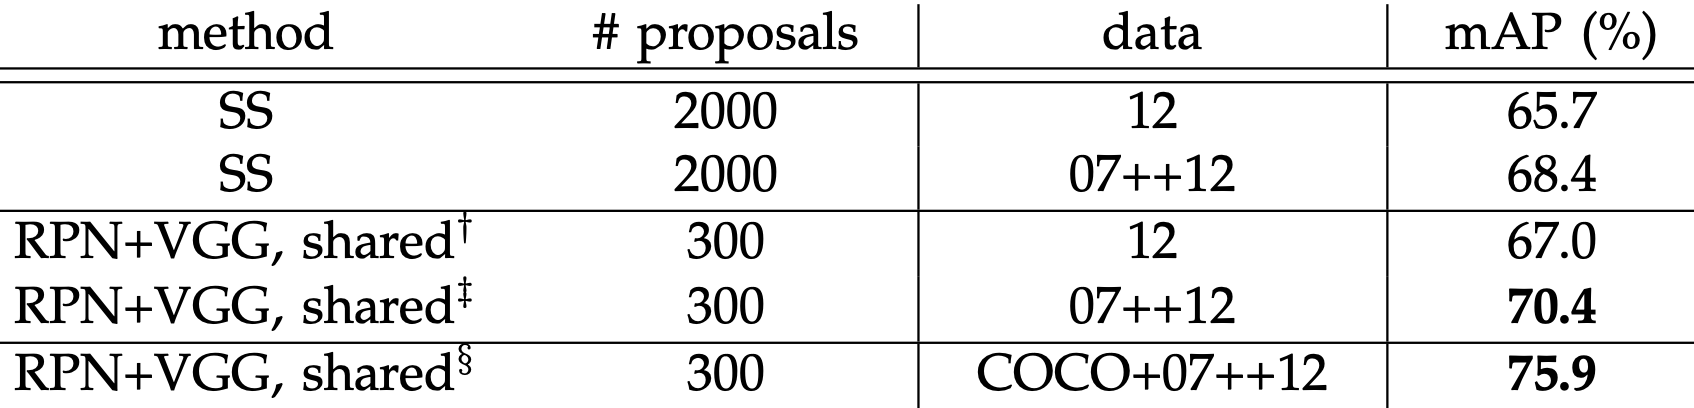
\includegraphics[width=10cm] {images/faster_rcnn_results_3}
    %     \caption{Kết quả của mô hình Fast R-CNN sử dụng RPN và backbone VGG-16 so sánh với mô hình Fast R-CNN sử dụng thuật toán Selective Search trên bộ dữ liệu VOC 2012 test với các bộ dữ liệu huấn luyện khác nhau. (Nguồn: \cite{ren2015faster})}
    %     \label{fig:faster_rcnn_results_3}
    % \end{figure}

    % \noindent
    % Cuối cùng, so sánh về mặt tốc độ, nhóm tác giả so sánh kết quả của các mô hình Faster R-CNN (dùng backbone là VGG-16, ký hiệu là \textbf{VGG, RPN + Fast R-CNN}), mô hình Faster R-CNN (dùng backbone là ZF-Net, ký hiệu là \textbf{ZF, RPN + Fast R-CNN}) với mô hình Fast R-CNN sử dụng thuật toán Selective Search (dùng backbone là VGG-16, ký hiệu là \textbf{VGG, SS + Fast R-CNN}).
    % Trong đó, thời gian (tính theo đơn vị ms) xử lý lớp conv được thống kê tại cột \textbf{conv}, thời gian đề xuất các khu vực được thống kê tại cột \textbf{proposals}, thời gian xử lý các bước như NMS, lớp pooling, lớp fully connected \index{lớp fully connected} và lớp softmax được thống kê tại cột \textbf{region-wise}, tổng thời gian xử lý toàn bộ được thống kê tại cột \textbf{total}, số lượng ảnh xử lý trong một giây được thống kê tại cột \textbf{rate}. \\
    % Kết quả, mô hình \textbf{VGG, RPN + Fast R-CNN} nhanh hơn \textbf{VGG, SS + Fast R-CNN} gần 10 lần, trong đó, thời gian đề xuất khu vực được tiết kiệm tới 150 lần.
    % Mô hình \textbf{ZF, RPN + Fast R-CNN} thậm chí còn nhanh gấp gần bốn lần mô hình \textbf{VGG, RPN + Fast R-CNN}, đạt số khung hình trên một giây là 17 fps.

    % \begin{figure}[H]
    %     \centering
    %     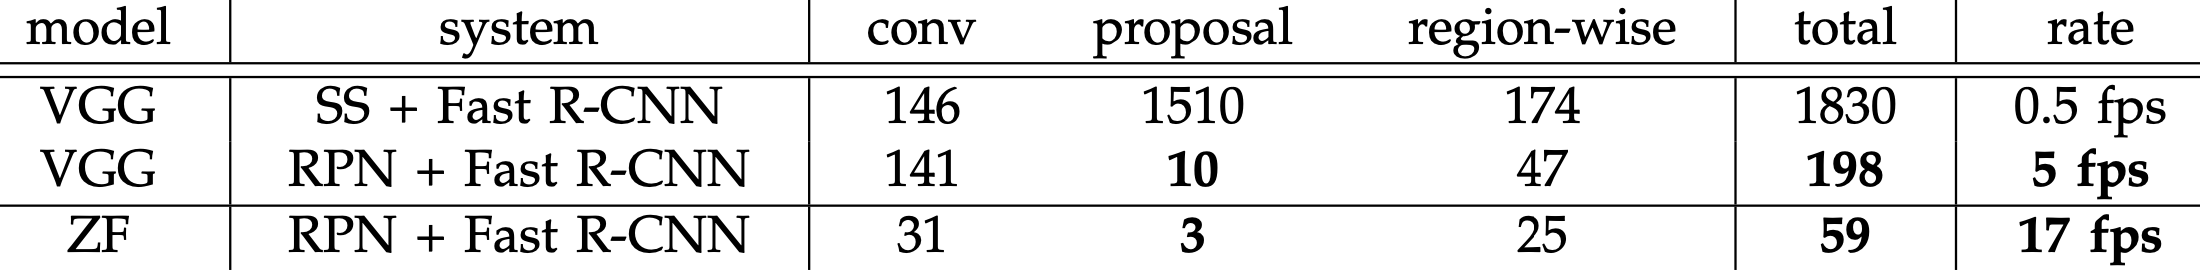
\includegraphics[width=10cm] {images/faster_rcnn_results_4}
    %     \caption{Toàn cảnh sự kết hợp của mô hình RPN và Fast R-CNN tạo ra mô hình Faster R-CNN (Nguồn: \cite{ren2015faster})}
    %     \label{fig:faster_rcnn_results_4}
    % \end{figure}

    \subsubsection{Vấn đề tồn đọng của mô hình Faster R-CNN}
    Kết quả của mô hình Faster R-CNN và tâm điểm là kiến trúc RPN giúp thay thế thuật toán Selective Search đã giúp cho Faster R-CNN đạt độ chính xác cao hơn so với mô hình Fast R-CNN sử dụng Selective Search.
    Hơn nữa, RPN giúp cho Faster R-CNN nhanh hơn tới 10 lần so với cấu hình tương tự Fast R-CNN sử dụng Selective Search.
    Điều này giúp cho Faster R-CNN cho đến nay vẫn là một mô hình tốt để giải quyết bài toán object detection, vừa đạt độ chính xác cao, vừa có tốc độ tương đối tốt.
    Tuy nhiên, cho đến thời điểm thực hiện luận văn này, đã có nhiều mô hình khác hiện đại hơn chỉ ra những vấn đề tồn đọng của Faster R-CNN như độ chính xác cần phải cải thiện thêm hay tốc độ chưa đạt đến ngưỡng chạy trong thời gian thực. 
}